\documentclass{sigchi}

% Use this command to override the default ACM copyright statement (e.g. for preprints). 
% Consult the conference website for the camera-ready copyright statement.


%% EXAMPLE BEGIN -- HOW TO OVERRIDE THE DEFAULT COPYRIGHT STRIP -- (July 22, 2013 - Paul Baumann)
% \toappear{Permission to make digital or hard copies of all or part of this work for personal or classroom use is         granted without fee provided that copies are not made or distributed for profit or commercial advantage and that copies bear this notice and the full citation on the first page. Copyrights for components of this work owned by others than ACM must be honored. Abstracting with credit is permitted. To copy otherwise, or republish, to post on servers or to redistribute to lists, requires prior specific permission and/or a fee. Request permissions from permissions@acm.org. \\
% {\emph{CHI'14}}, April 26--May 1, 2014, Toronto, Canada. \\
% Copyright \copyright~2014 ACM ISBN/14/04...\$15.00. \\
% DOI string from ACM form confirmation}
%% EXAMPLE END -- HOW TO OVERRIDE THE DEFAULT COPYRIGHT STRIP -- (July 22, 2013 - Paul Baumann)


% Arabic page numbers for submission. 
% Remove this line to eliminate page numbers for the camera ready copy
\pagenumbering{arabic}


% Load basic packages
\usepackage{balance}  % to better equalize the last page
\usepackage{graphics} % for EPS, load graphicx instead
\usepackage{times}    % comment if you want LaTeX's default font
\usepackage{url}      % llt: nicely formatted URLs

% llt: Define a global style for URLs, rather that the default one
\makeatletter
\def\url@leostyle{%
  \@ifundefined{selectfont}{\def\UrlFont{\sf}}{\def\UrlFont{\small\bf\ttfamily}}}
\makeatother
\urlstyle{leo}


% To make various LaTeX processors do the right thing with page size.
\def\pprw{8.5in}
\def\pprh{11in}
\special{papersize=\pprw,\pprh}
\setlength{\paperwidth}{\pprw}
\setlength{\paperheight}{\pprh}
\setlength{\pdfpagewidth}{\pprw}
\setlength{\pdfpageheight}{\pprh}

% Make sure hyperref comes last of your loaded packages, 
% to give it a fighting chance of not being over-written, 
% since its job is to redefine many LaTeX commands.
\usepackage[pdftex]{hyperref}
\hypersetup{
pdftitle={SIGCHI Conference Proceedings Format},
pdfauthor={LaTeX},
pdfkeywords={SIGCHI, proceedings, archival format},
bookmarksnumbered,
pdfstartview={FitH},
colorlinks,
citecolor=black,
filecolor=black,
linkcolor=black,
urlcolor=black,
breaklinks=true,
}

% create a shortcut to typeset table headings
\newcommand\tabhead[1]{\small\textbf{#1}}


% End of preamble. Here it comes the document.
\begin{document}

\title{The Quanti-CHI-ed Self: A Data Driven Analysis of the Structure of Research Communities at the CHI 2013 Conference.}

\numberofauthors{3}
\author{
  \alignauthor Anant Bhardwaj\\
    \affaddr{MIT CSAIL}\\
    \email{anantb@csail.mit.edu}\\
 \alignauthor Juho Kim\\
    \affaddr{MIT CSAIL}\\
    \email{juhokim@mit.edu}\\
\alignauthor Haoqi Zhang\\
    \affaddr{Northwestern University}\\
    \email{hq@northwestern.edu}\\
\alignauthor David Karger\\
    \affaddr{MIT CSAIL}\\
    \email{karger@mit.edu}\\
\alignauthor Sam Madden\\
    \affaddr{MIT CSAIL}\\
    \email{madden@csail.mit.edu}\\
}


\maketitle

\begin{abstract}
CHI has traditionally supported diverse and interdisciplinary work and continues to expand into new topics not previously explored.  While many of us have opinions about the distribution of interests in this community, there has been little data available to support these opinions.

At CHI 2013, 630 attendees used the myCHI interactive conference program to select the papers they considered of interest to see or attend.  We use this data to understand the CHI 2013 community structure --- specifically, the sub-areas of interest and the connections between them. We believe the data and our analysis demonstrate how the CHI community can better understand its own structure and use this knowledge in planning future conferences and community interactions. The data can also be useful in discovering new areas of research and practice, new methodologies, and emerging application areas.
\end{abstract}

\keywords{
        CHI Community Structure; myCHI; 
}

\category{H.5.m.}{Information Interfaces and Presentation (e.g. HCI)}{Miscellaneous}

\section{Introduction}
A primary role of academic conferences is to bring together people with shared interest to exchange ideas and knowledge.  It thus seems crucial to understand whether and how attendees are connected by shared interests.  Understanding the structure of shared interests can help in scheduling sessions, choosing speakers, creating program committees, and helping people get to know others with similar interests.  

To date, such interests structures have been inferred primarily by hearsay.  In this note, we argue that and show how it is possible to use data gathered from conference attendees to quantify our understanding of the CHI community structure -- to apply the “quantified self” perspective to our own community.  We consider conferences as a collaborative activity that can benefit from CSCW approaches.   We identify subcommunities with shared interests -- some apparently so strong that are almost a separate “conference within a conference”-- that might benefit from greater recognition or autonomy within CHI.  We take the position that gathering such data more aggressively prior to CHI 2014 could allow us to enhance the quality of CHI 2014 by structuring sessions better, by scheduling shared-interest events, and by better-choosing invited speakers, and could enhance the quality of future CHIs by informing us about the proper arrangement of subcommittees (submission tracks).

Our analysis uses data from myCHI, a “conference program app” for desktop and mobile that gave attendees a list and schedule of talks and allowed them to “star” those talks they wanted to attend or otherwise found interesting.  Of the 3400 CHI attendees, 630 used myCHI to star an average of 25 papers each.  We use these stars as an indication of the interests of different attendees.  We cluster papers and attendees based on these shared interests, and use the clusters to understand major “sub-areas” of CHI and the degree of connection between them.

Over the years, CHI~\cite{chi2013} has strived to maintain diversity, balance, collaboration and evolution. There is a set of conference-defined core communities that have persisted over several years including User Experience, Design, Engineering, and Management. These core communities seek to cover HCI as a discipline, and are overlapping. Each year, CHI also has a different set of \emph{featured communities} which are more domain-oriented to provide an environment in which community members can incubate and grow a new community.  CHI 2012~\cite{chi2012} had several featured communities including Health, Games and Entertainment, Sustainability, Child-Computer Interaction, and Digital Arts. CHI 2013~\cite{chi2013} evolved by adding HCI for Development as a new community to the list.

We are aware that our data, which covers only 1/5 of the attendees, is biased.  However, we believe this data suffices to (i) demonstrate the existence of communities that are not explicitly recognized as CHI Communities and (ii) demonstrate how much more could be done with a concerted effort to gather this data from a larger portion of the attendees.

This paper is organized into three major parts. In the first part, we very briefly describe the myCHI system and how attendees used myCHI at CHI 2013. In the second part we present the data we collected, and an analysis of the data. We analyze the data at different zoom levels to see if it illuminates us with new information. The third part is a discussion on what is the implication of our analysis on the CHI community at large. Before concluding we take a brief digression to discuss why we chose not to include certain kinds of data in our analysis and the possible risks associated with it.


\section{MyCHI}
myCHI is a tool for conference attendees to plan their conference. Conference attendees can search for a keyword and mark papers they find interesting. 

As soon as a user marks at least one paper as interesting, the system starts recommending more papers similar to ones the user has marked as interesting. This way, the user can create a personalized list of all the papers he or she wants to see in the conference. 
 

\begin{figure}[!h]
\centering
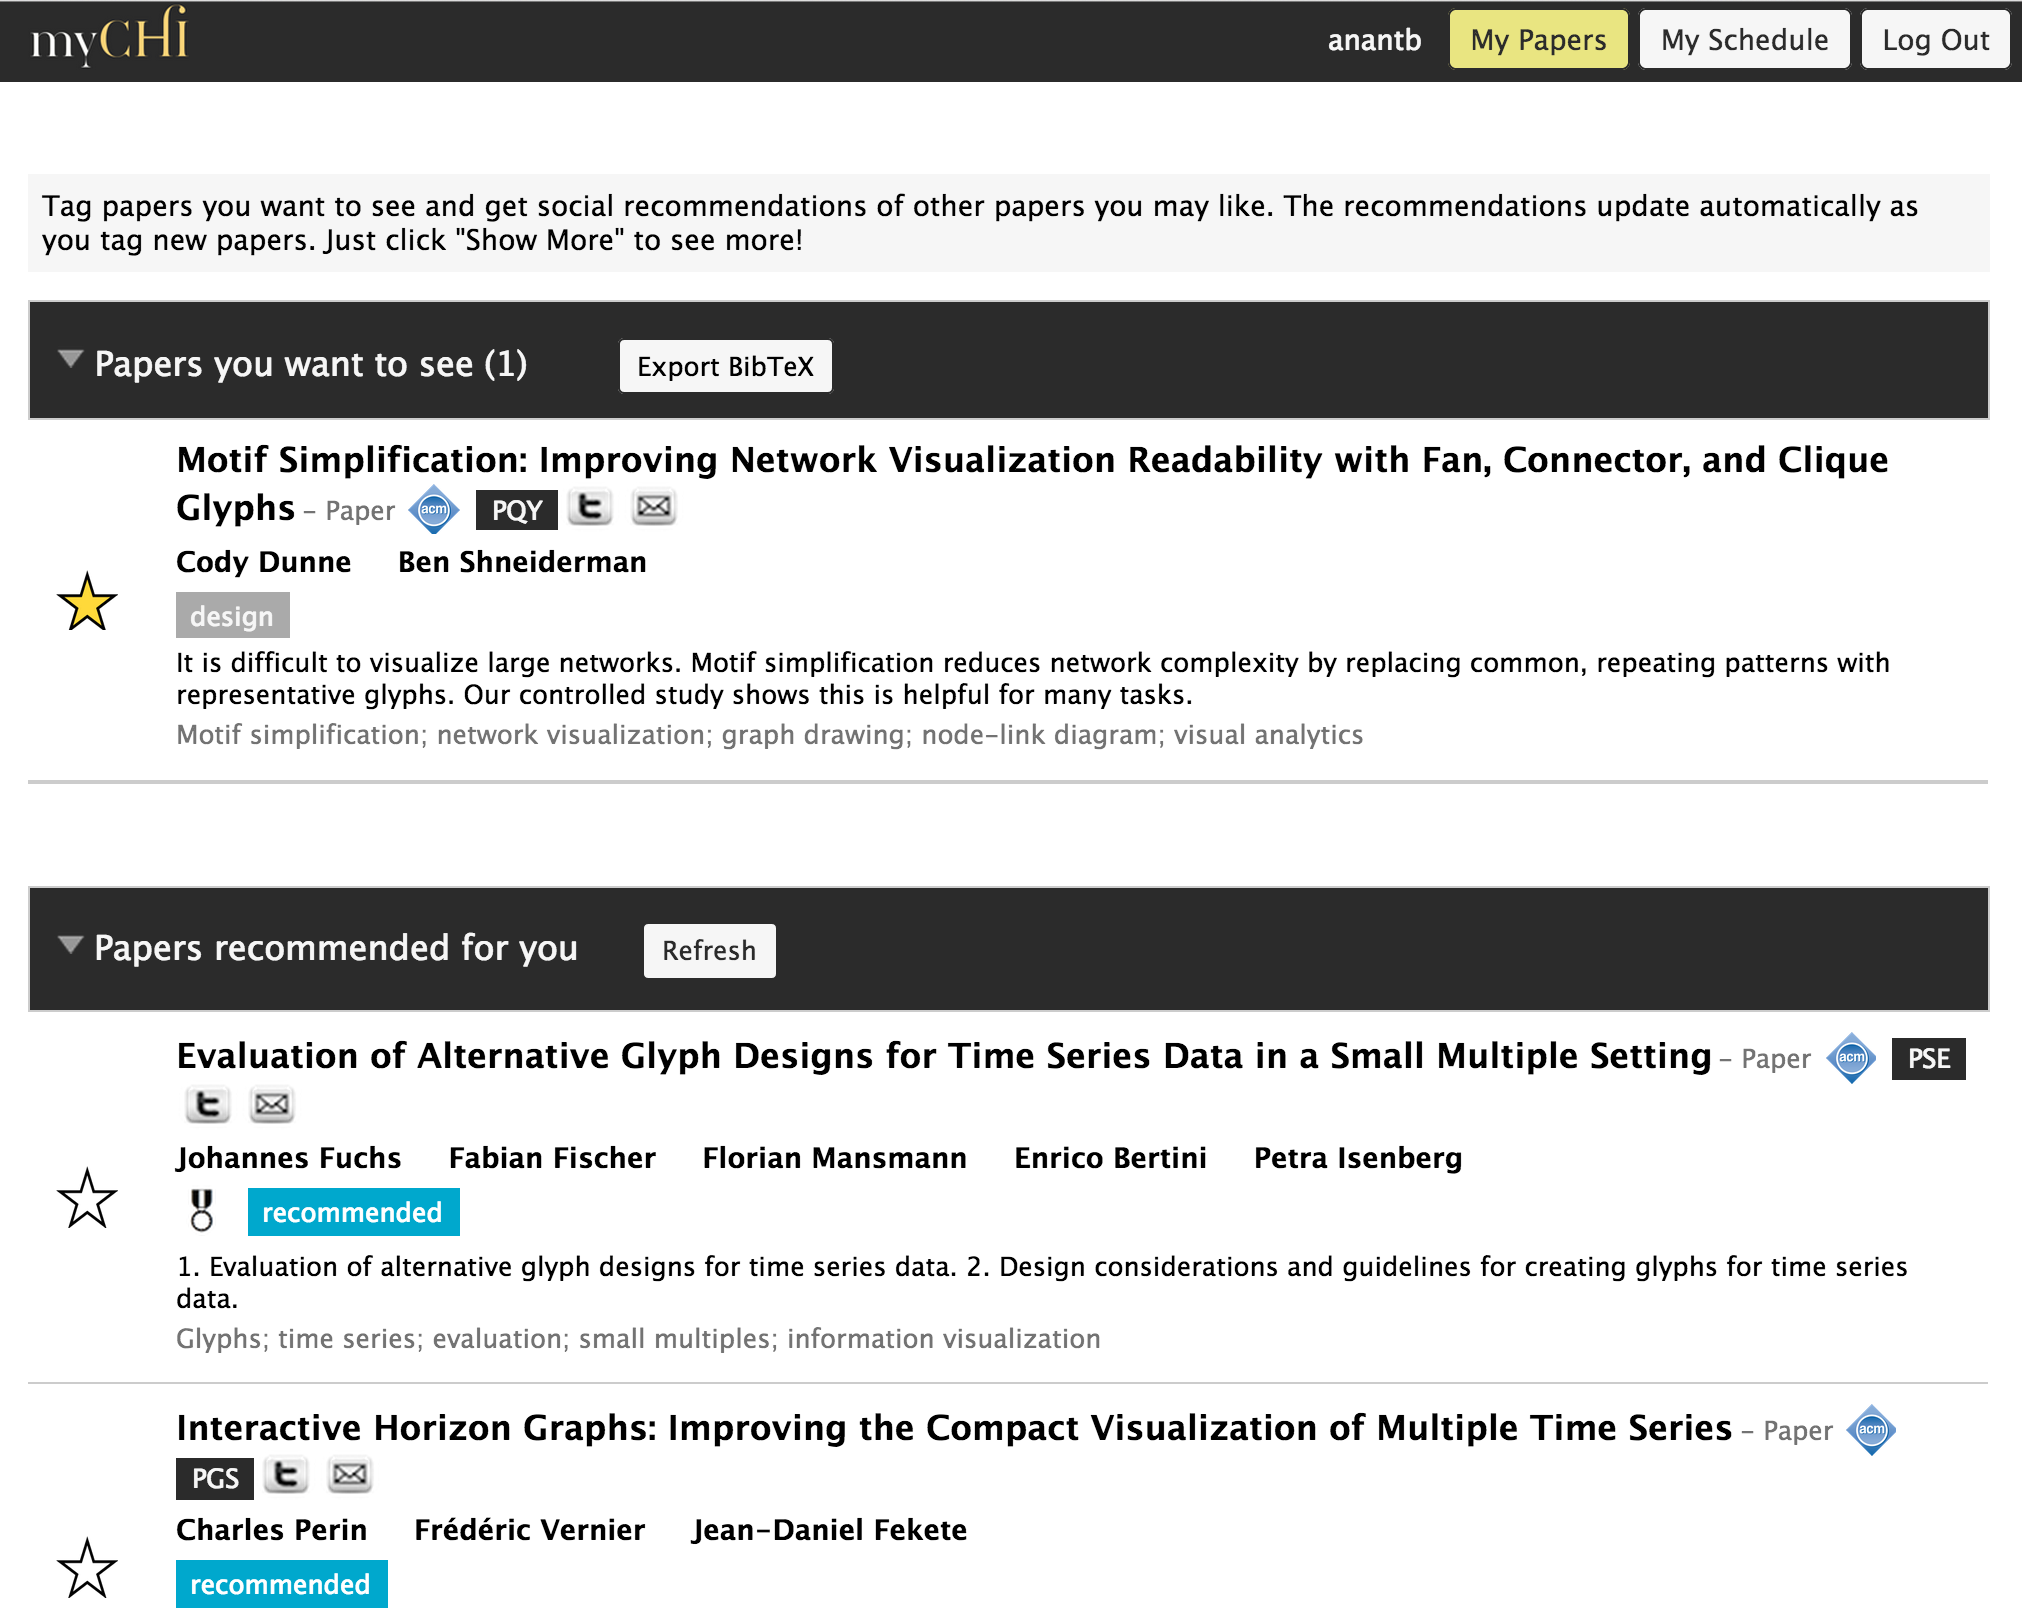
\includegraphics[width=0.9\columnwidth]{mychi-papers-view-recommendations}
\caption{My Paper View -- the top section shows all the starred papers, the middle section shows all the recommended papers, and the bottom section (not visible in the figure) shows all the papers.}
\label{fig:MyCHI -- My Papers}
\end{figure}

Our recommendation system uses collaborative filtering to recommend new papers and thus the recommendations are based on what other people with a similar set of interests have in their personalized list. For CHI 2013, we used cobi~\cite{Zhang:2013:CCL:2468356.2479597} generated preference list to bootstrap the system so that our initial recommendations aren't biased.

\begin{figure}[!h]
\centering
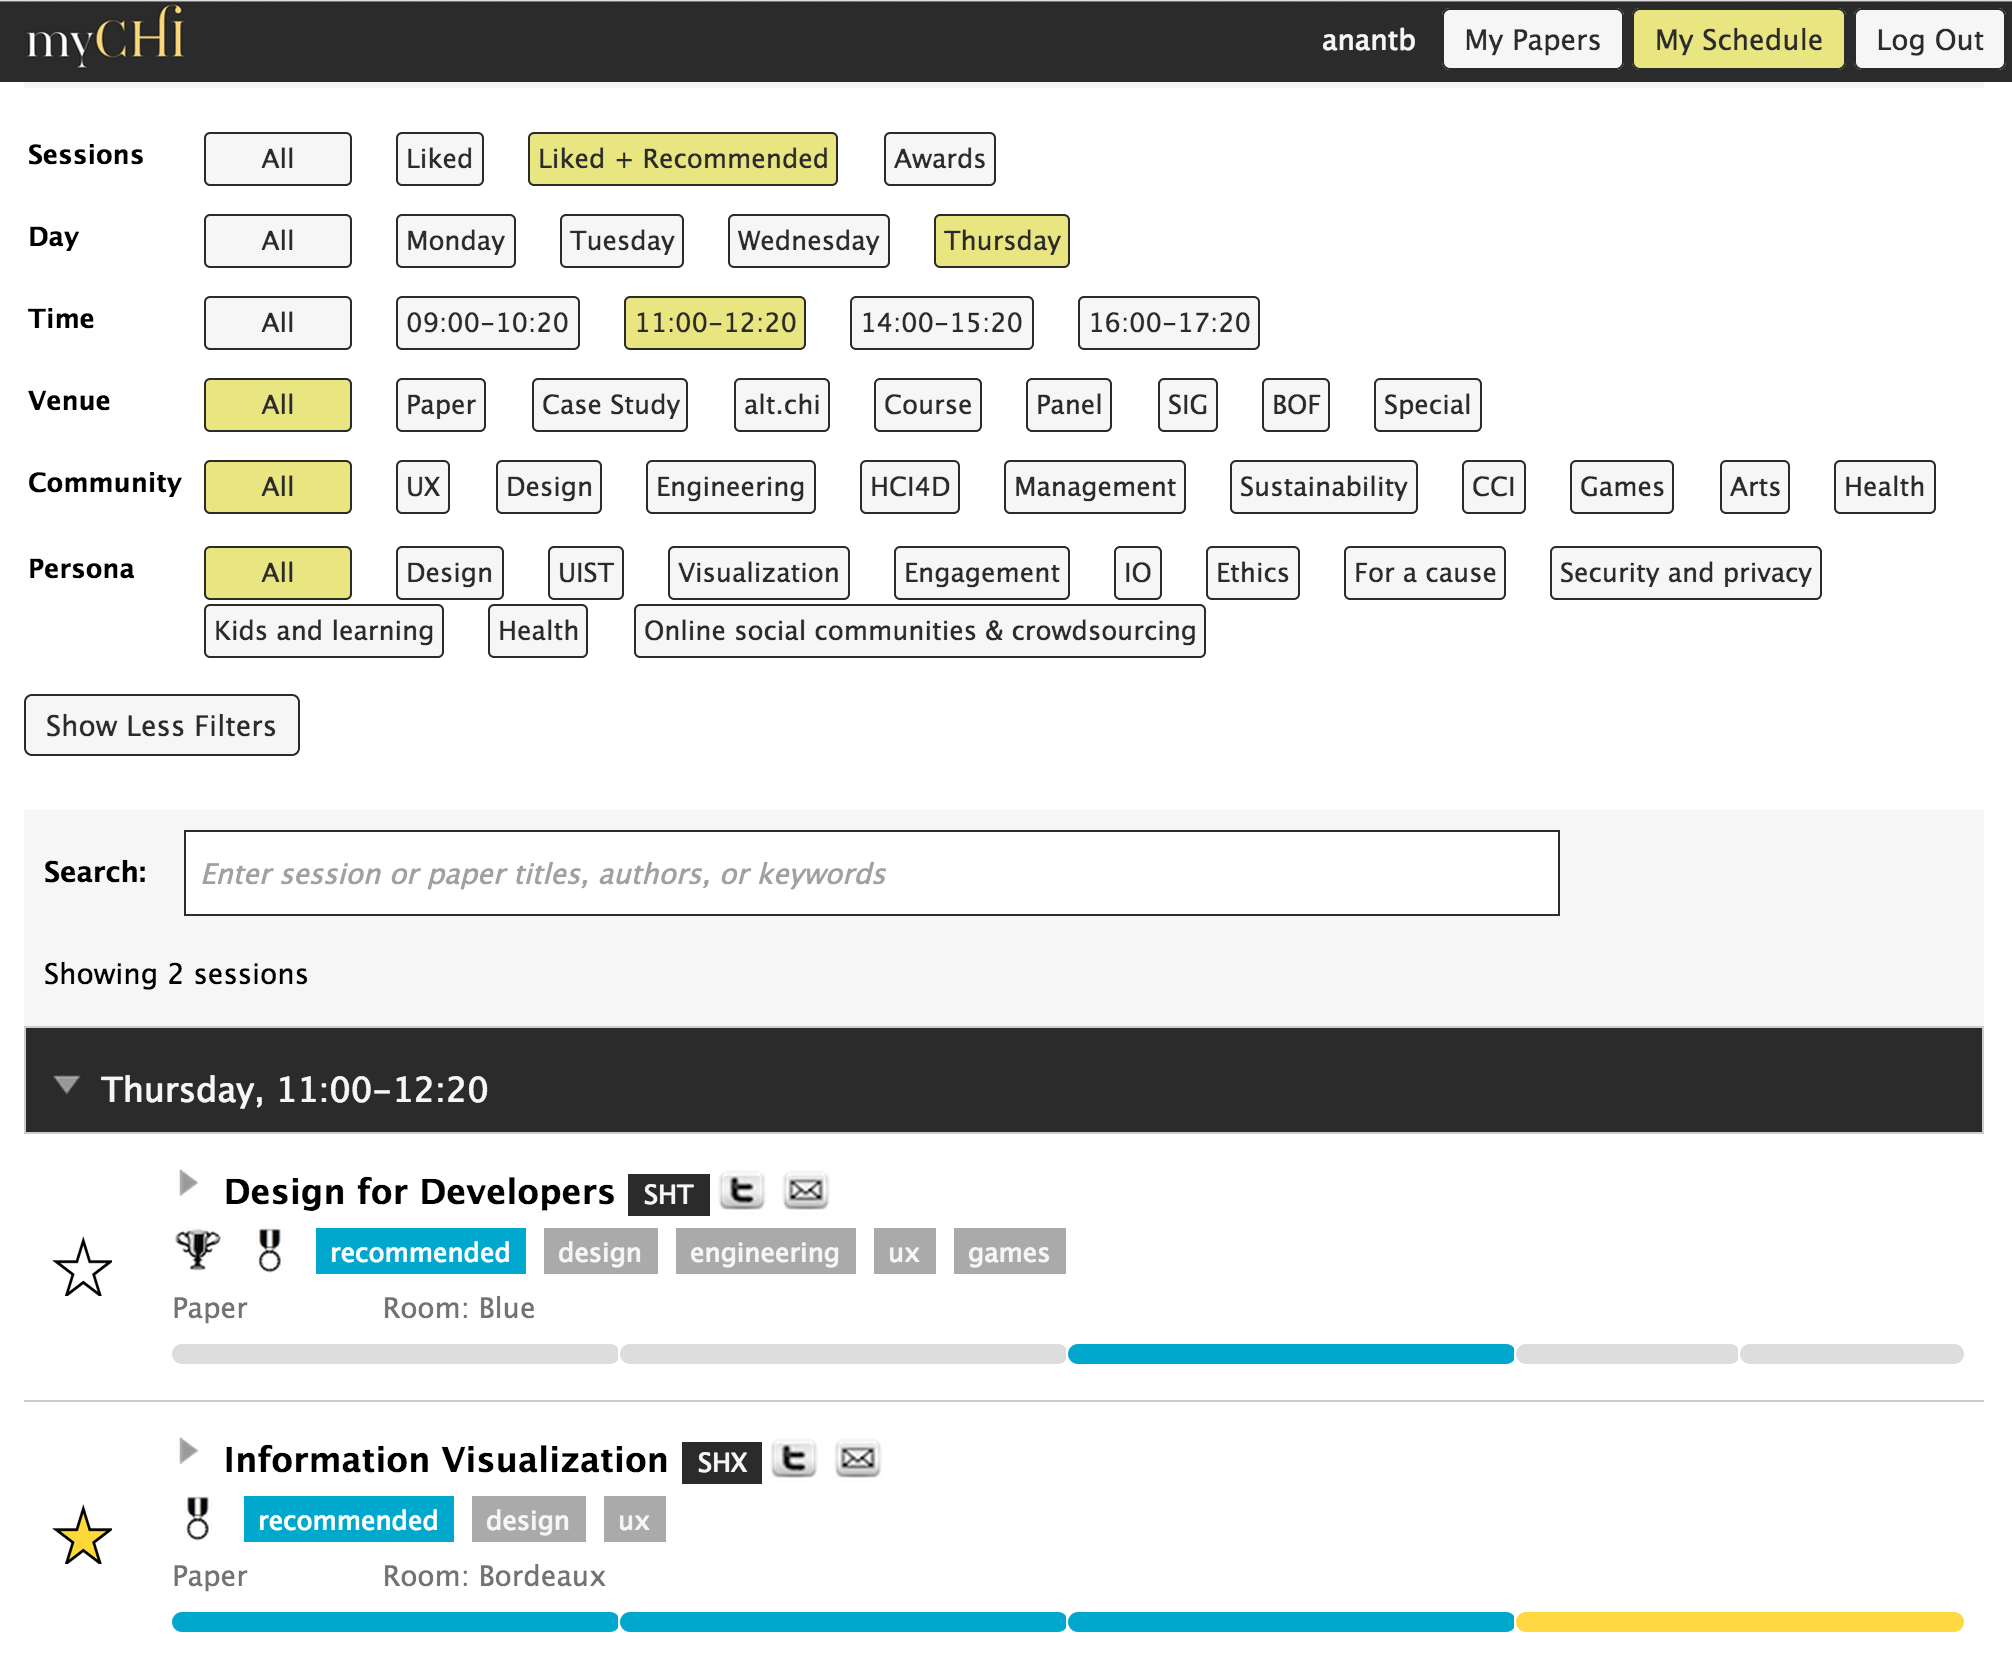
\includegraphics[width=0.9\columnwidth]{mychi-schedule-view}
\caption{My Schedule View -- a set of filters to easily navigate through the conference schedule.}
\label{MyCHI -- My Schedule}
\end{figure}

To incentivize users to use myCHI, we recommend a personalized schedule to each user which helps the user navigate through the conference. This personalized schedule is created based on all the papers the user has starred, and the papers recommended by our recommendation system based on his or her preferences. We provide a set of filters that allows users to see different views of their personalized schedule and make an informed decision of where they should spend their time. Fig. 2 shows myCHI schedule view.


\section{MyCHI Data and Analysis}
\subsection{Usage Statistics}
Before we present an analysis, we present usage statistics. We dropped all the users with 0 starred papers from our analysis. There were total of 630 users who starred at least 1 paper. The avg. number of starred papers per user was 20.6 (std. Dev: 22.7, median: 13,  min: 1, max 155). The avg. number of people starring a paper was 24.2 (std. Dev: 12.1, median: 22,  min: 1, max 80). Every paper presented in the conference was starred by at least 1 person. 

\begin{figure}[!h]
\centering
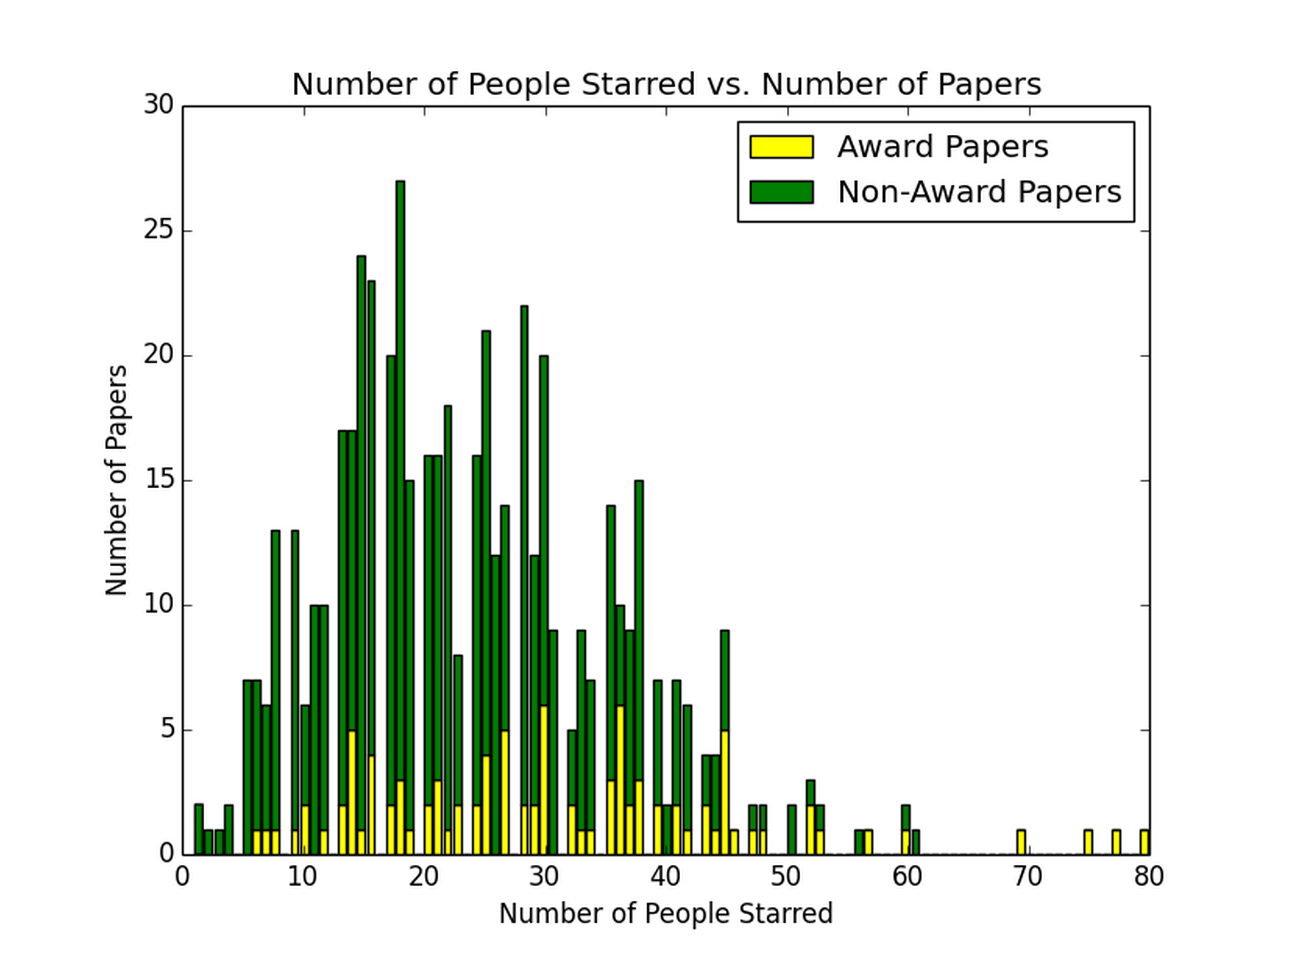
\includegraphics[width=0.9\columnwidth]{papers_likes}
\caption{A histogram plot of Popularity of Papers}
\label{fig:A histogram plot of Number of People Starred (any single paper)}
\end{figure}



\subsection{Award Papers}

To understand if the papers popular on myCHI were the award and honorable mention (hm) papers, we compute the popularity stats for award and honorable mention papers. For award and honorable mention papers, the average popularity (``number of people selecting the paper") goes up by 26\% (mean: 30.97, std dev: 15.3, median: 30.0 min: 6, max: 80). For award only papers, these numbers improve a bit more (mean: 33.3, std dev: 17.3,  median: 29.5, min: 6, max: 77)---a 37\% increase.

While we see that award/hm papers have better average popularity,  there are papers that were very popular on myCHI ( more than 50 stars) but they were not part of award/hm papers. Out of 14 papers that got more than 50 stars, only 9 of them were part of award/hm papers (approximately 35\% of popular papers were not part of award/hm papers). Also, there are quite a few award/hm papers (see the plot) for which the popularity was less than the overall average.





\subsection{Community Analysis}
\footnote[1]{Links to these visualizations: http://double-blind.org/mychi}
A community is a set of people with a common area of interest. We wanted to understand whether clear subcommunities exist at CHI, or whether the community is an undifferentiated whole.  This is a clustering problem. We could have focused on clustering people based on shared interest in papers, but it is difficult to inspect a given person and understand their interests.  So we instead chose to cluster papers, which have meaningful titles, based on shared people.  We created a graph where each node represents a paper, and two papers are connected by an edge if the number of people interested in both exceeds some threshold X..  We will vary X below.   For visualization, we clustered the graph's nodes using force-directed~\cite{Eades00navigatingclustered} drawing.

This allows us to understand communities at different zoom levels. At very low common interest (X = 5), almost the entire graph is connected and that shows all of CHI as a single community. As we increase X, we see different communities within CHI. Below is a graph with a common interest threshold 10 (there is an edge between two nodes if and only if at least 10 people have starred both the papers). At this level three strong communities appear within CHI.  One on the right, containing 57 papers about hardware (multi-touch, gesture, tabletop, sensing surfaces), is quite isolated.  On the left are two clusters more closely coupled: at the bottom, a cluster of 39 papers on crowds, social media, and education, and above it, a cluster of 37 papers on design.  These three clusters together contain 133 papers, more than 1/3 of the total at the conference.  We will defer our discussion on the isolated nodes until next subsection.


An important task in conference preparation is to assign papers to sessions that hopefully reflect the relationships between the papers.  To visually explore this, we labeled each node (represents a paper) with its session\_id (a unique id assigned to the session at which this paper was presented).  Examining the graph, one can see that almost all the papers within a session are part of the same cluster, suggesting that sessions were well-chosen. 


\begin{figure}[!h]
\centering
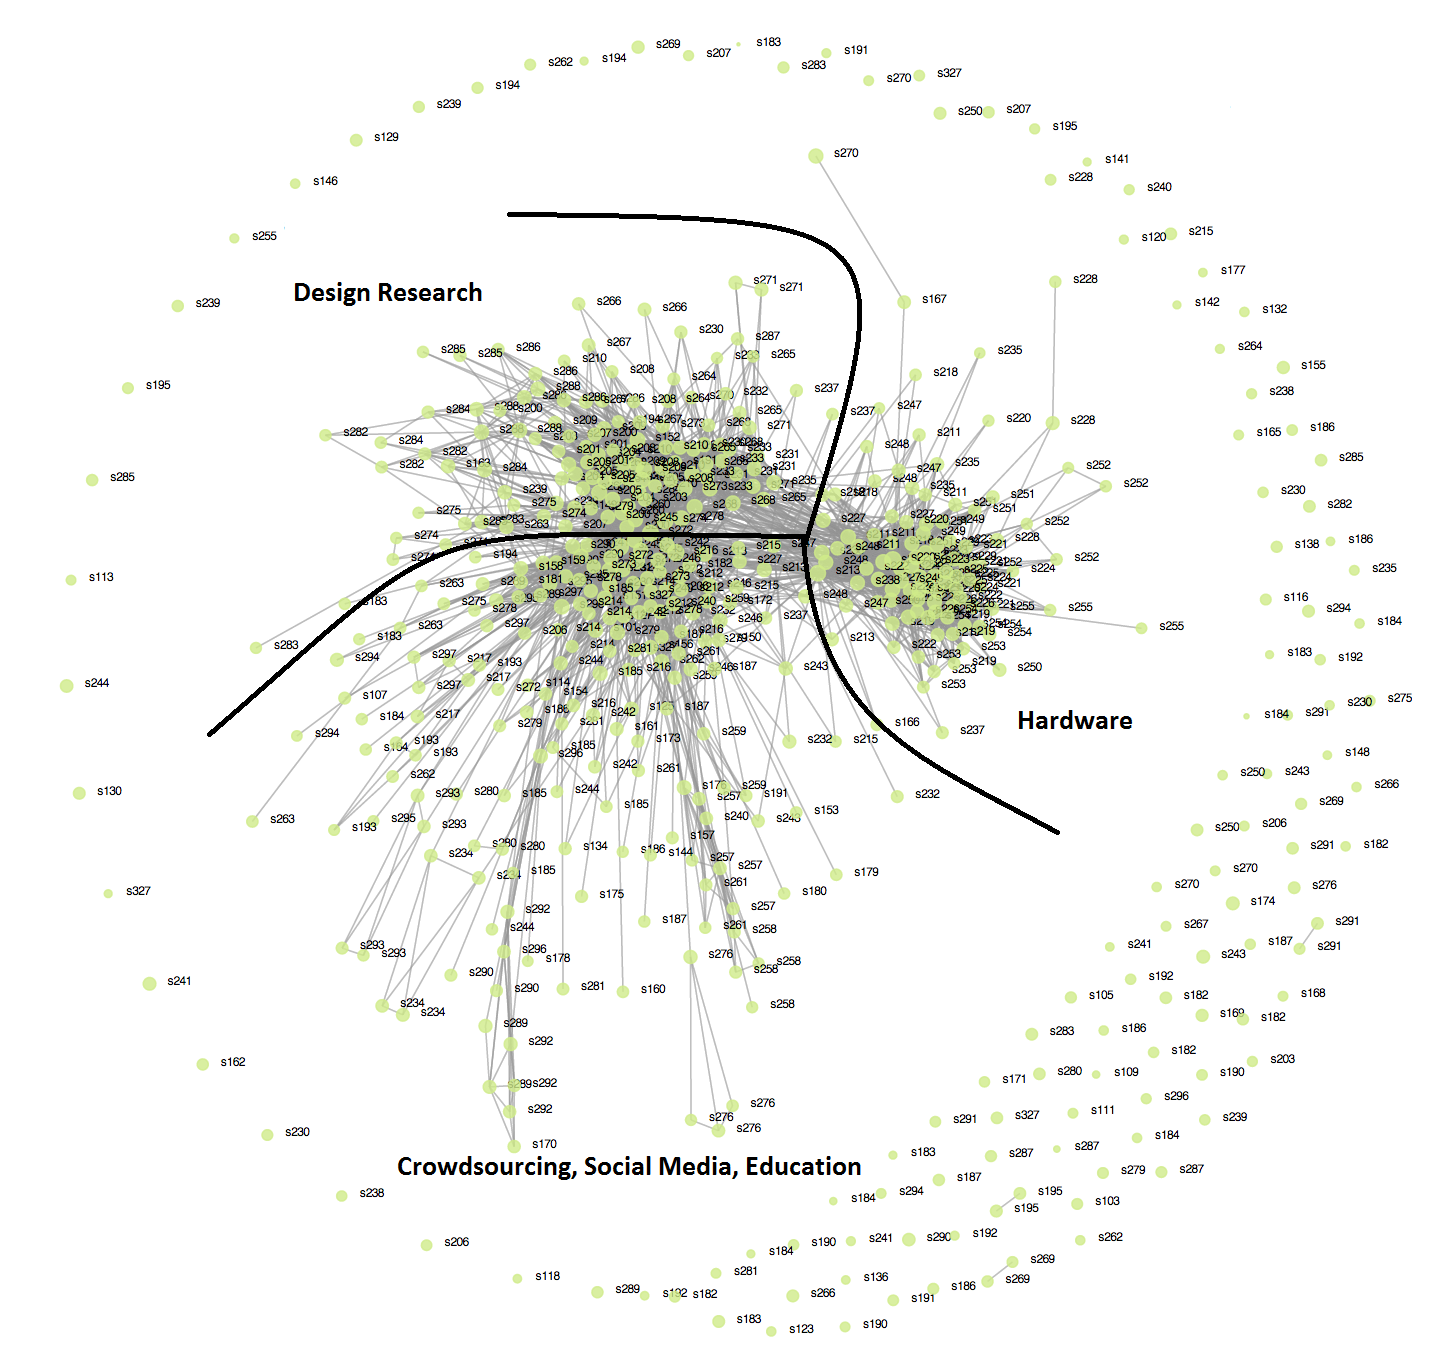
\includegraphics[width=0.9\columnwidth]{mychi-community-view-10}
\caption{A cluster of papers based on a common interest threshold 10 (there is an edge between two nodes if and only if at least 10 people have starred both the papers). A force-directed drawing creates a cluster of densly connected nodes. }
\label{fig:Community View of threshold 10}
\end{figure}

To further refine our understanding of the community structure, we increase the common interest threshold to 15 (there is an edge between two nodes if and only if at least 15 people have starred both the papers). This reveals six different communities. At this point hardware community remains densely packed but new communities emerge from the second and the third clusters. Now, the second cluster has new communities like crowdsourcing, social media, education, and information visualization. The third cluster gets divided into communities like design research and participatory design. Also, there are some strongly connected isolated subgraphs that separated out from the two larger clusters are health, games, gesture etc.




\begin{figure}[!h]
\centering
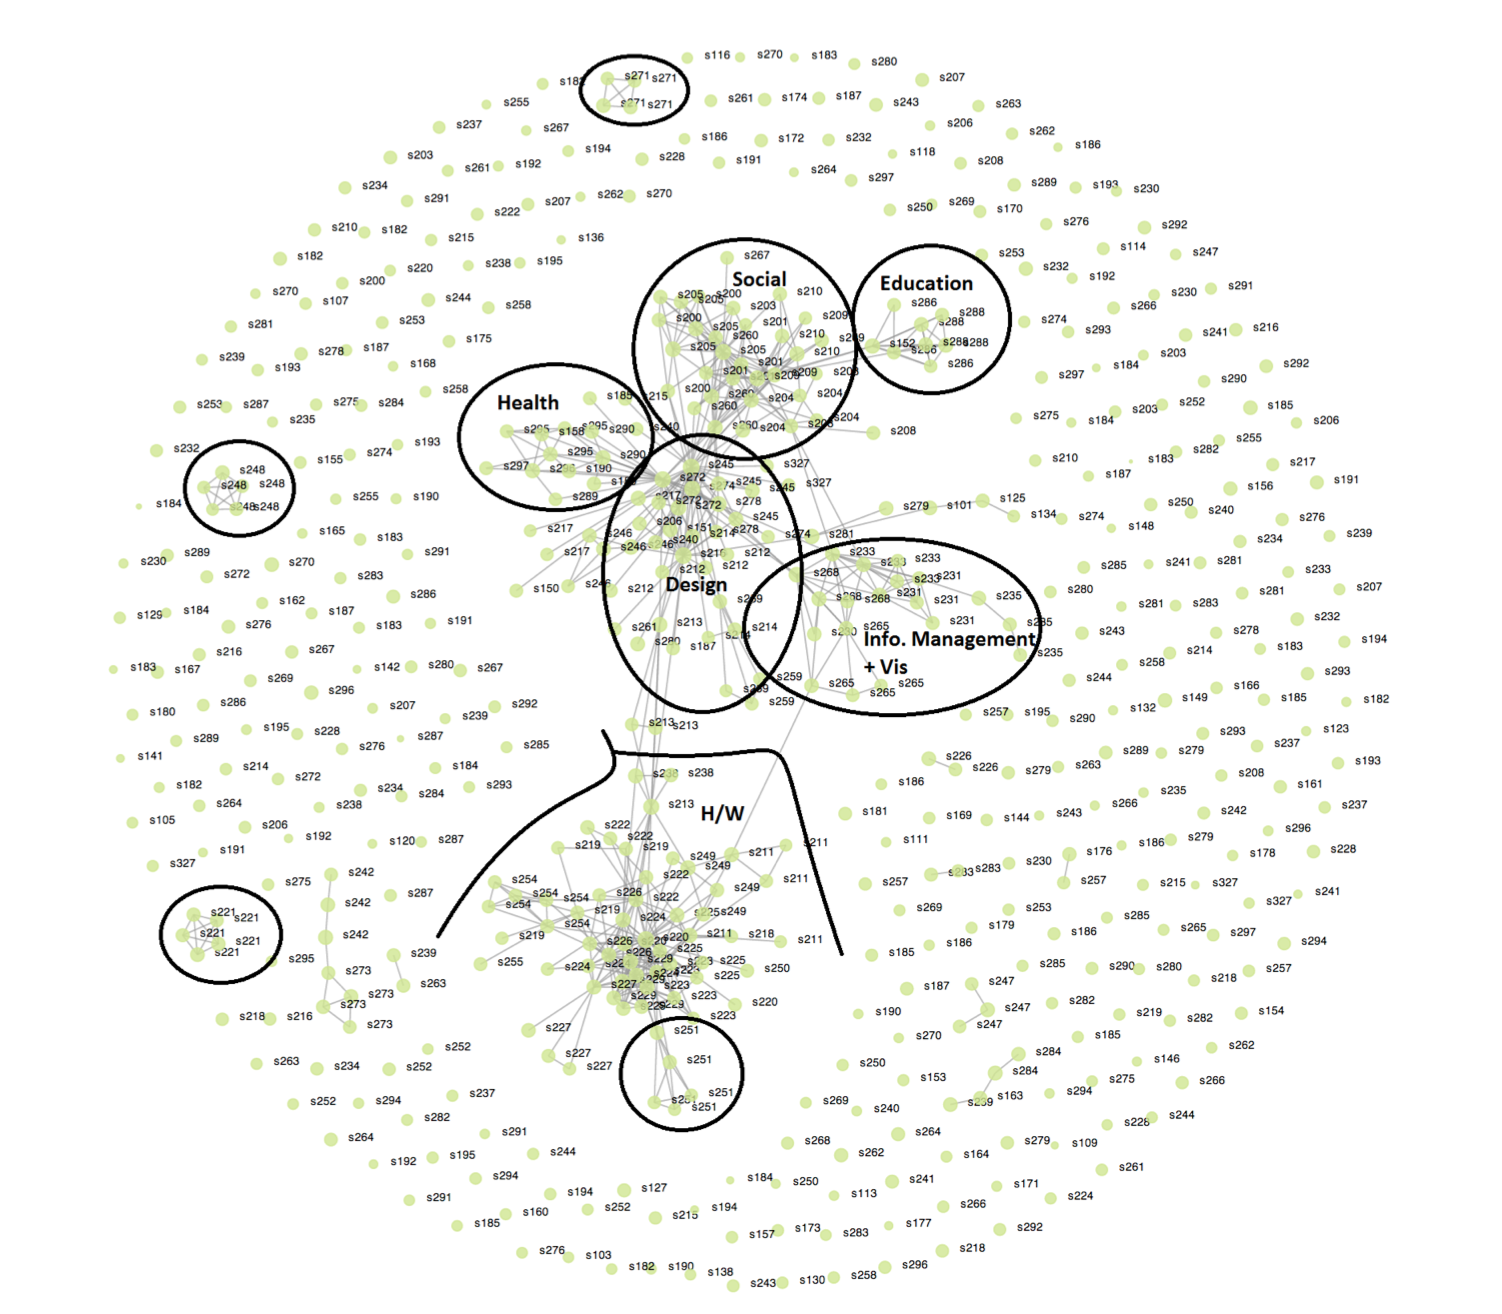
\includegraphics[width=0.9\columnwidth]{mychi-community-view-15}
\caption{A cluster of papers based on a common interest threshold 15 (there is an edge between two nodes if and only if at least 15 people have starred both the papers). A force-directed drawing creates a cluster of densly connected nodes. }
\label{Community View of threshold 15}
\end{figure}

As we see from the above two graphs, there are more isolated nodes as we increase the threshold of common interest to detect the clusters. If we lower the threshold of common interest then the established communities dominate and all nodes become part of some established community.  In order to recognize emerging clusters, we removed all the connected subgraphs (all the established communities) from Fig. 5, and re-clustered the remaining nodes with a lower common interest threshold. Because of space constraints, we are not able to put another visualization but new communities such as accessibility, rural development, pointing devices, multi touch, gesture, etc. emerged from that exercise.




\section{Discussion}
The preliminary analysis carried out here suggests that there is significant community sub-structure at CHI that is not really reflected at the organizational level.  While CHI formally labels a community around “Design”, it offers no corresponding community around Social Media, or around the incredibly tight Hardware community.  Indeed, the Hardware community seems so densely connected that it might benefit from more autonomy, perhaps running its own events or its own program committee under the CHI umbrella.  

As we stated above, it is clear that data from only 1/5 of attendees cannot give a complete picture of interests at the conference.  But this could easily be improved.  Were the CHI organizers to explicitly pursue gathering this data prior to holding (or scheduling) the conference, then a far higher rate of data gathering could be achieved, especially if attendees understood that it could make the conference better for them.  Paper preference lists would provide invaluable data for scheduling, ensuring that sessions drew together individuals with shared interests, and that conflicts between papers with the same audience were minimized.  Once communities of interest were identified for a given year (possibly unrelated to other years), panels and birds-of-a-feather gatherings could be organized to discuss the papers and topics of greatest interest to that subcommunity.  Communities of interest that persisted over many years could be granted more autonomy within the CHI conferences, reducing the coordination burden at the top.  

\subsection{Deeper Analysis and Risks}
We have restricted our analysis to group scale because mis-use of the data may lead to undesirable perturbations in the quantities being measured. Clearly, it would infringe on privacy to report on individual users.  But there are even risks in reporting on individual papers. Readers will note that we have not reported obvious facts in our possession such as the most popular papers overall or per cluster. Our reasoning is as follows: as soon as the data is analyzed to reflect positively on a specific paper, people will face a motivation to game the system to their own benefit.  For example, if we begin reporting popular papers, then authors might be motivated to ask friends to mark his or her paper as interesting, whether or not it truly is, simply to attain more visibility for the paper.   We may already face a similar risk at the group scale, where our reporting on clusters/interest groups may motivate members of a group to ``link farm", promising to ``like" each others' papers in order to increase the apparent density and importance of their own group.  However, we believe that risks are substantially higher at the individual level, so have chosen to limit our analysis to the group level.

Looking ahead, this may well be a matter to be tackled by the CHI community leadership.  What should our community policy be on the reporting of these kind of statistics?  Should the policy be different for an academic setting such as this one compared to e.g. a pure-entertainment ``popularity contest" at the conference itself? We do have statistics on the most popular papers, and providing that information could be of value to the community in understanding where it is headed.  If the program committee argues for it, we could include that information in the revision of this submission.





\section{Conclusion}

myCHI is a tool that collects natural, rich preference data on how attendees plan to spend their time at the conference. This data provides information on the communities' interests and substructure, emerging sub-communities, and interactions within a community and between communities. We use this dataset to analyze how CHI 2013 attendees' interests are distributed over different topic areas, the strength of different established communities, and emerging communities. At very high level we see two broader communities at CHI -- hardware community and everything else. Once we zoom in, we observe that the non-hardware community gets clustered into crowdsourcing, education, social media, design, information visualization, etc. The hardware community also spawns sub-communities like gesture, multitouch etc. We try to dig deeper by removing the influence of stronger communities and we observe emerging communities like pointing devices, accessibility, analytics, etc.  Many of these communities are officially recognized at CHI, while some of them are scattered over multiple communities. While we defer from making strong claims, we believe that the data-driven technique can discover the latent community structure and thus can help in refining the CHI community structure. It can influence how sessions are planned, and how subcommunities are formed to enable better communication and reduce conflicts. Also, the organically emerging communities and subcommunities reflect the future direction of where CHI is heading to as a community.



% Balancing columns in a ref list is a bit of a pain because you
% either use a hack like flushend or balance, or manually insert
% a column break.  http://www.tex.ac.uk/cgi-bin/texfaq2html?label=balance
% multicols doesn't work because we're already in two-column mode,
% and flushend isn't awesome, so I choose balance.  See this
% for more info: http://cs.brown.edu/system/software/latex/doc/balance.pdf
%
% Note that in a perfect world balance wants to be in the first
% column of the last page.
%
% If balance doesn't work for you, you can remove that and
% hard-code a column break into the bbl file right before you
% submit:
%
% http://stackoverflow.com/questions/2149854/how-to-manually-equalize-columns-
% in-an-ieee-paper-if-using-bibtex
%
% Or, just remove \balance and give up on balancing the last page.
%
\balance

\bibliographystyle{acm-sigchi}
\bibliography{mychi}
\end{document}
